\subsection{Variants and Variant Calling} \label{background:variants_and_variant_calling}
When examining the genome of several individuals within the same species, one will find locations along the genome where the nucleotides differ for the different individuals.
These distinct nucleotide manifestations are commonly referred to as \textit{variants}.
The term \textit{variant calling} is used to refer to the process of determining which variants an individual has.
In other words, given a reference genome sequence, where and how does the genome sequence of the individual of interest differ from the reference sequence.
This process can abstractly be described in three steps: 
1) sequence the genome of interest to get DNA reads (described in section \ref{background:high_throughput_dna_sequencing}), 
2) align the reads to the reference genome by finding where along the reference genome sequence each read fits best, usually using a heuristic determining which location the read originates from, and 
3) examine the alignments and note where and how the reference and the individual's sequences differ to determine the variants present in the individual's genome \cite{variant_calling}.

A common way to represent genome sequence variations is to encode them according to the \textit{Variant Call Format} (VCF) file format.
The VCF file format encodes a single variant per line, and each line contains a number of columns where each column encodes a particular piece of information about the associated variant, such as \cite{vcf}:
\begin{compactenum}
  \item
    CHROM: an identifier for the reference sequence used, \textit{i}.\textit{e}. the sequence against which the sequenced reads varies.
  \item
    POS: the position along the reference sequence where it varies against the sequenced reads.
  \item
    ID: an identifier for the variantion.
  \item
    REF: the reference base (or bases) found at the POS position in the reference sequence.
  \item
    ALT: a list of the alternative base (or bases) found at this POS position.
\end{compactenum}
While more columns are usually present, this encapsulated the necessary knowledge about variants and their representation needed for this thesis.

\definecolor{variantcolor}{RGB}{235,235,235}

\begin{figure}[H]
\begin{center}
\scalebox{1}{
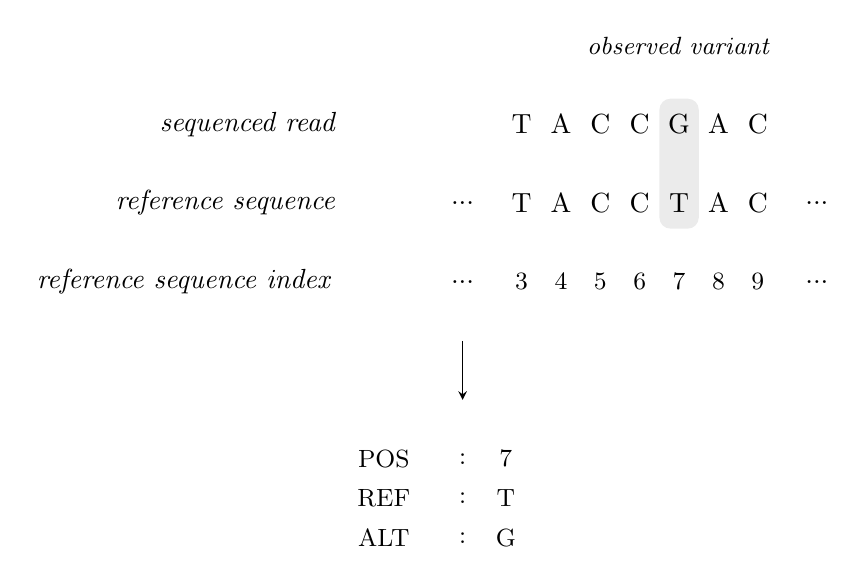
\begin{tikzpicture}
  % texts
  \node at(2.75,2)(title){\small{\textit{observed variant}}};
  \node at(-3.525,-1)(title){\textit{reference sequence index}};
  \node at(-3,0)(title){\textit{reference sequence}};
  \node at(-2.715,1)(title){\textit{sequenced read}};
  % color boxes
  \node at(2.75,0.5)[rounded corners,minimum width=0.5cm,minimum height=1.65cm, fill=variantcolor](variant){};
  % indices
  \node at(0,-1)(n1){$...$};
  \node at(.75,-1)(n2){\small{3}};
  \node at(1.25,-1)(n3){\small{4}};
  \node at(1.75,-1)(n4){\small{5}};
  \node at(2.25,-1)(n5){\small{6}};
  \node at(2.75,-1)(n5){\small{7}};
  \node at(3.25,-1)(n5){\small{8}};
  \node at(3.75,-1)(n5){\small{9}};
  \node at(4.5,-1)(n5){$...$};
  % lower nodes
  \node at(0,0)(n1){$...$};
  \node at(.75,0)(n2){T};
  \node at(1.25,0)(n3){A};
  \node at(1.75,0)(n4){C};
  \node at(2.25,0)(n5){C};
  \node at(2.75,0)(n5){T};
  \node at(3.25,0)(n5){A};
  \node at(3.75,0)(n5){C};
  \node at(4.5,0)(n5){$...$};
  % upper nodes
  \node at(.75,1)(n2){T};
  \node at(1.25,1)(n3){A};
  \node at(1.75,1)(n4){C};
  \node at(2.25,1)(n5){C};
  \node at(2.75,1)(n5){G};
  \node at(3.25,1)(n5){A};
  \node at(3.75,1)(n5){C};
  % down arrow
  \draw [-stealth](0,-1.75) -- (0,-2.5);
  % POS 
  \node at(-1,-3.25)(vcf_pos){\small{POS}};
  \node at(0,-3.25)(vcf_pos){\small{:}};
  \node at(0.55,-3.25)(vcf_pos){\small{7}};
  % REF
  \node at(-1,-3.75)(vcf_ref){\small{REF}};
  \node at(0,-3.75)(vcf_ref){\small{:}};
  \node at(0.55,-3.75)(vcf_ref){\small{T}};
  % ALT
  \node at(-1,-4.25)(vcf_alt){\small{ALT}};
  \node at(0,-4.25)(vcf_alt){\small{:}};
  \node at(0.55,-4.25)(vcf_alt){\small{G}};
\end{tikzpicture}
}
\caption{An illustration of how a sequenced read can be aligned to a reference sequence and the variant present in the sequenced read is determined and encoded in (a simplified) VCF format, where several of the common columns are omitted.}
\label{background:variant_and_variant_calling:figures:variants}
\end{center}
\end{figure}

